\section{Eredmények}
A vizsgálatok menete tipikusan úgy zajlik, hogy szintetikus \textit{"kvázi-kísérleti"} adatokat állítunk elő: Összeállítottunk két idegsejtmodellt -- egy egykompartmentumos, amely egyetlen szómából áll és egy \textit{"Ball and Stick"} modellt, amely pedig egy szómához csatlakozó dendritből áll -- és ennek az adott modellparaméterek melletti áramlépcső stimulusra adott válaszfüggvényére zajt  raktunk, így szimulálva a kísérleti adatokat. Majd ezekre az adatokra végeztük el a paraméterbecslést. Ezzel a módszerrel vizsgálni tudjuk az inferencia pontosságát, mert ismerjük a kiinduló, \textit{"igazi"} paramétereket. Minden esetben passzív idegsejtmodellekkel dolgoztunk.

Ugyanazokat a becsléseket -- új kezdeti paraméterek és zaj megvalósulásokra -- sokszor elvégeztük és a következő, inferencia minőségét jellemző statisztikákat állítottuk fel rájuk:
\begin{enumerate}
	\item \textbf{Eltérés \textit{(diff)}}: Az inferencia során becsült paraméter mennyire van távol az eredeti, kiindulási paramétertől.
	\item \textbf{Pontosság \textit{(acc)}}: A becsült paraméter poszterior eloszlásának maximuma (legvalószínűbbnek becsült paraméter valószínűsége, azaz maximális valószínűség) hányszorosa a kiindulási (eredeti) paraméterértékhez társított valószínűségnek: $p_{true}/p_{max}\cdot 100$.
	\item \textbf{Élesség \textit{(gain)}}: A poszterior eloszlás hányszor élesebb a priornál: $\Pi_{s}/P_s$. Ez természetesen akkor jellemzi a különböző eseteket, ha ugyanakkora prior eloszlással számolunk. Az eloszlás élességét úgy vizsgáljuk, hogy a görbe csúcsától a feléig veszünk egyenletesen $50$ magasságpontot -- illetve függvényértéket $y$ --, amikhez tartozó $x$-értékek -- ebből kettő van ideális esetben, mert a normál eloszlás szimmetrikus -- távolságát összegezzük, majd normáljuk $50$-el az eredményt.
	Ez az egyik legfontosabb jellemző, mert arra nyújt betekintést, hogy a mérés mennyi új információt hordozott.
%	\item \textbf{Laposság \textit{(broadness)}}: $P_{s}/\Pi_s\cdot 100$. Ezt az mennyiséget azért érdemes bevezetni, mert nagyon kis $P_s$ értékeknél az élességhez tartozó érték \textit{"elszáll"}, így nagy lesz a szórása. Szemléletesen azt jelenti, hogy ha ez az érték $100\%$ akkor a poszteriorom épp olyan mint a priorom, tehát nem nyertem ki új információt a kísérletből.
\end{enumerate}

Ezeket a statisztikákat elvégeztük különböző modellekre -- különböző zajmodellek mellett -- és kísérleti protokollokra, melynek eredményeit a következő pontokban részletezzük. Végezetül valódi kísérleti adatokra is alkalmaztuk a paraméterbecslési eljárásunkat, valamint vizsgáltuk a kísérleti zaj tulajdonságait.



\subsection{Egykompartmentumos modell}
Először a \ref{sec:single-comp}-fejezetben tárgyalt passzív egykompartmentumos modellre alkalmazzuk a megoldásainkat. Egy pontszerű szómát ingerlünk áramimpulzus bemenettel, valamint mérjük a feszültségválaszát. Ennek szemléltetése látható a \ref{fig:point}-ábrán.

\begin{figure}[h!]
	\centering
	\includegraphics[width=0.4\linewidth]{fig/models/point}
	\caption[Egykompartmentumos modell szemléltetése]{Egykompartmentumos modell szemléltető ábrája. Egyetlen pontszerű -- nincs térbeli kiterjedés -- szómát stimulálunk az elektróda árammal és mérjük a feszültségválaszát.}
	\label{fig:point}
\end{figure}

Egy $175 \left[ms\right]$-on keresztül injektált $0.1 \left[mA\right]$ áramerősség stimulusú -- és passzív biofizikai beállítású -- protokollt alkalmaztunk az alábbiakban. Továbbá a fehér zaj szórásának mindenhol $\sigma_w = 7\left[mV\right]$-ot választottunk. Hasonló beállításokkal előállított adatsor tekinthető meg a korábbi \ref{fig:white}-ábrán. Színes zaj szórásának pedig $\sigma_\epsilon = \sqrt{3} \left[mV\right]$-ot és az időbeli korreláció lecsengési idejét jellemző karakterisztikus idejének pedig $\tau=10 \left[ms\right]$-ot. Ezt szemlélteti a korábbi \ref{fig:colored}-ábra.

\subsubsection{Fehér zaj}
\paragraph{egy paraméter}
Az a kérdés, hogy passzív egykompartmentumos modell áramlépcső stimulusra adott feszültségválasza segítségével, milyen pontosan tudunk egy paramétert -- jelen esetben a $cm$ membránkapacitás paraméterét -- becsülni.

Az eredmények a \ref{fig:wn1}-ábrán láthatóak. A legfontosabb jellemző mennyiség az élesség, amely jelen esetben $2.75$-nek adódott. Ez azt jelenti, hogy szimulációk során a poszterior eloszlás átlagosan $2.75$-ször élesebb (hegyesebb) volt a prior eloszlásnál. A mérés után ennyi új információra tehetünk szert az adott paraméterre nézve.


\paragraph{két paraméter}
Itt azt vizsgáljuk, hogy együtt inferálva $cm$ paramétert egy másik ($g_{pas}$) paraméterrel, az mennyire befolyásolja a $cm$ becslését.

A \ref{fig:wn2_joint}-ábrán látható egy futtatás tipikus eredménye a két paraméter együttes poszterior eloszlására. Ebből látszódik, hogy $g_{pas}$ paraméter nagyon pontosan becsülhető, ennek következtében nem rontja le a másik ($cm$) paraméter becslését. Másképp fogalmazva az együttes eloszlás, szinte épp maga a $cm$ paraméter marginális eloszlása. 


A \ref{fig:wn2}-ábrán látható a sok futtatás eredményéből származó marginális eloszlások és statisztikák mindkét paraméterre. Ezeken látszódik, hogy $g_{pas}$ paraméter eloszlása tényleg nagyon éles, a priorjánál $15.87$-szer élesebb a poszteriorja. Tehát ezt a paramétert pontosan tudjuk becsülni. Továbbá az is látható, hogy a $cm$ paraméter marginális poszterior eloszlásának alakja valóban lényegesen nem változott, nem romlott a becslés pontossága -- a fentebbi meggondolásokkal egybevágóan.

\subsubsection{Színes zaj}
A kétparaméteres becslést exponenciálisan lecsengő autokorrelációval rendelkező színes zaj esetére is elvégeztük. Azt várjuk, hogy a becslés pontossága csökkenni fog, mivel az adatpontok nem függetlenek, így kevesebb effektív mintavételi pontunk van -- még akkor is, ha növeljük az időbeli felbontását.

A paraméterek együttes eloszlása a \ref{fig:cn1_joint}-ábrán láthatóak. Összehasonlítva a fehér zajos esettel ez tényleg kevésbé éles. A \ref{fig:cn1}-ábrán pedig a sok szimuláció átlagos, egyes paraméterekre marginalizált eredménye látható.

Az eredmények azt mondják, hogy valóban pontatlanabb a becslés színes zaj esetén, hiszen mindkét paraméter \textit{élessége} csökkent: $cm$-nek $1.92$ és $g_{pas}$-nak pedig $7.66$. És mindezt úgy, hogy ráadásul kisebb ($\sigma_\epsilon = \sqrt{3} \left[mV\right]$) szórást alkalmaztunk mint fehér zajnál ($\sigma_w = 7\left[mV\right]$)!

\begin{figure}[h!]
	\centering
	\subfloat[Illusztráció]{{\includegraphics[width=0.5\textwidth]{./fig/wn1/illustration_cm.png} }}
	\subfloat[Élesség]{{\includegraphics[width=0.5\textwidth]{./fig/wn1/igain_cm.png} }}
	\\	
	\subfloat[Eltérés]{{\includegraphics[width=0.5\textwidth]{./fig/wn1/deviation_cm.png} }}
	\subfloat[Pontosság $(p_{max}/p_{true}\cdot 100)$]{{\includegraphics[width=0.5\textwidth]{./fig/wn1/accuracy_cm.png} }}
	\caption[Egy kompartmentum, egy paraméter, fehér zaj eredmény és ábratípus magyarázat]{$100$ db szimuláció összefoglaló ábrái az egyparaméteres, fehér zajos becsléshez. Az \textbf{(a)} rész illusztrálja a szimulációk során előforduló átlagos poszterior alakot, valamint egyéb statisztikákat is feltüntet: A fejlécen láthatóak (sorban) az \textbf{eltérés}(diff), \textbf{pontosság}(acc) és \textbf{élesség}(gain) átlagos értékei. Továbbá a függőleges zöld sáv azt jelzi, hogy a valódi érték milyen tartományban mozgott, ha ezt a poszteriort kaptuk. Vagy épp ellenkezőleg úgy is felfoghatjuk, hogy ha a prior csúcsánál van a valódi érték, akkor a becsült poszterior maximuma a zöld sávban mozgott szimulációk során. Végül a vízszintes kék sáv azt mutatja, hogy a valódi értékekhez milyen valószínűségeket rendelt a poszterior általában -- ez konzisztens az előzővel. Az előbbiek szépen szemléltetik a valószínűségi felfogást: a poszterior alatti tartományomban lesz valahol az igazi érték, de nem biztos, hogy a maximális valószínűségnél. \textbf{(b)}, \textbf{(c)} és \textbf{(d)} ábrarészleteken pedig az előbbi értékek hisztogramos ábrázolása látható.}
	\label{fig:wn1}
\end{figure}

%\begin{figure}[h!]
%	\centering
%	\subfloat[Fehér zajos együttes eloszlás]{{\includegraphics[width=0.5\textwidth]{./fig/wn2/JointP_cm_gpas(1).png} }}
%	\subfloat[Színes zajos együttes eloszlás]{{\includegraphics[width=0.5\textwidth]{./fig/cn1/JointP_cm_gpas(1).png} }}
%	\caption[(Egy kompartmentum két paraméter, fehér zaj eredmény]{\textbf{(a):} Egy futtatásból származó kétparaméteres, fehér zajos inferencia együttes eloszlása. Láthatóan $g_{pas}$ paramétert nagyon pontosan tudjuk becsülni, $cm$ paramétert pedig kevésbé. \textbf{(b): Előbbihez hasonló }}
%	\label{fig:joints}
%\end{figure}


\begin{figure}[h!]
	\centering
	\includegraphics[width=0.8\linewidth]{fig/wn2/JointP_cm_gpas(1).png}
	\caption[Egykompartmentumos modell fehér zaj együttes poszterior eloszlása]{Egy futtatásból származó kétparaméteres, fehér zajos becslés együttes eloszlása. Láthatóan $g_{pas}$ paramétert nagyon pontosan tudjuk becsülni, $cm$ paramétert pedig kevésbé.}
	\label{fig:wn2_joint}
\end{figure}


\begin{figure}[h!]
	\centering
	\subfloat[$cm$ paraméter]{{\includegraphics[width=0.5\textwidth]{./fig/wn2/illustration_cm.png} }}
	\subfloat[$g_{pas}$ paraméter]{{\includegraphics[width=0.5\textwidth]{./fig/wn2/illustration_gpas.png} }}
	\caption[Egy kompartmentum két paraméter, fehér zaj eredmény]{$100$ db szimuláció összefoglaló ábrái a kétparaméteres, fehér zajos becslésre, külön mind a két paraméterre. Ezek már a szimuláció során előforduló, átlagos marginális poszterior eloszlásalakok az egyes paraméterekre.}
	\label{fig:wn2}
\end{figure}


\begin{figure}[h!]
	\centering
	\includegraphics[width=0.8\linewidth]{fig/cn1/JointP_cm_gpas(1).png}
	\caption[Egykompartmentumos modell, színes zaj, együttes poszterior eloszlása]{Egy futtatásból származó kétparaméteres, színes zajos becslés együttes eloszlása. Látható, hogy a paramétereket kevésbé pontosan tudjuk becsülni, mint a fehér zajos esetben.}
	\label{fig:cn1_joint}
\end{figure}

\begin{figure}[h!]
	\centering
	\subfloat[$cm$ paraméter]{{\includegraphics[width=0.5\textwidth]{./fig/cn1/illustration_cm.png} }}
	\subfloat[$g_{pas}$ paraméter]{{\includegraphics[width=0.5\textwidth]{./fig/cn1/illustration_gpas.png} }}
	\caption[Egy kompartmentum, két paraméter, színes zaj eredmények]{$100$ db szimuláció összefoglaló ábrái a kétparaméteres, színes zajos becslésre, külön mind a két paraméterre. Ezek már a szimuláció során előforduló, átlagos marginális poszterior eloszlásalakok, az egyes paraméterekre.}
	\label{fig:cn1}
\end{figure}




\clearpage
\subsection{Térbelileg kiterjedt modell: \textit{Stick and Ball}}
A \ref{sec:multi-comp}-fejezetben tárgyalt térbelileg kiterjedt, többbkompartmentumos passzív idegsejtmodellekre is alkalmaztuk a módszerünket. Pontosabban a \textit{Ball and Stick} modellre, amely egy szómához csatlakozó dendritből áll. A szómába injektáltuk az elektróda áramot és azon is mértünk. Ennek szemléltetése látható a \ref{fig:spatial}-ábrán.

\begin{figure}[h!]
	\centering
	\includegraphics[width=0.9\linewidth]{fig/models/spatial}
	\caption[Többkompartmentumos modell szemléltetése]{Térbelileg kiterjedt, \textit{Stick and Ball} modell szemléltető ábrája. Egy szómához csatlakozik egy dendrit, melyet kisebb kompartmentumokra bontunk ($D1,D2,...$). A szómát ingereljük és azon is végzünk mérést.}
	\label{fig:spatial}
\end{figure}

Az $R_a$ és $g_{pas}$ paramétereket becsüljük együtt. Azt várjuk, hogy a dendritere jellemző passzív paraméter ($R_a$), azaz a fajlagos axiális ellenállás meghatározása kevésbé pontos lesz, tisztán a szómán végzett mérésekből, előzetes ismereteink alapján.

Itt is egy $175 \left[ms\right]$-on keresztül injektált $0.1 \left[mA\right]$ áramerősség stimulusú protokollt alkalmaztunk, ugyancsak passzív biofizikai és hasonló zaj beállításokkal.


\subsubsection{Fehér zaj}
Hasonlóan az előző pontokban látottakhoz, erre az összeállításra is lefuttattuk a szimulációkat. Az egy futtatásból származó tipikus együttes likelihood függvény és poszterior eloszlás látható a \ref{fig:wn3_joint}-ábrán, valamint a sok futtatás eredménye pedig a \ref{fig:wn3}-ábrán.

Az eredmények teljesen kielégítik az elvárásainkat: az $R_a$ paraméter tényleg rosszul becsülhető tisztán az idegsejten végzett mérésekből és ez egyben (valamennyivel) rontja $g_{pas}$ paraméter becslését is. Az együttes eloszlások ábrájáról látszódik jól, hogy ez miért történik: az $Ra-gpas$ paramétersíkra levetített ellipszisek kissé \textit{"ferdék"}, így $R_a$ tengelyre kiösszegezve az eloszlást, $g_{pas}$ marginális eloszlása kiszélesedik. Előfordulhat olyan eset, hogy az egyik paramétert rosszul tudjuk becsülni, viszont ez a másikat nem rontja el -- tehát a paraméterek nem \textit{"korrelálnak"} --, akkor ha a levetített ellipszisek nem ferdék.


\begin{figure}[h!]
	\centering
	\subfloat[együttes likelihood]{{\includegraphics[width=0.5\textwidth]{./fig/wn3/JointL_Ra_gpas(0).png} }}
	\subfloat[együttes poszterior]{{\includegraphics[width=0.5\textwidth]{./fig/wn3/JointP_Ra_gpas(0)} }}
	\caption[\textit{Stick and ball}, két paraméter, fehér zaj együttes eloszlásai]{Egy (fehér zajos) futtatásból származó likelihood(a) és poszterior(b). Szépen látszódik, hogy az $R_a$ paraméter becslése tényleg pontatlan, míg a $g_{pas}$ továbbra is viszonylag éles.}
	\label{fig:wn3_joint}
\end{figure}


\begin{figure}[h!]
	\centering
	\subfloat[$R_a$ paraméter]{{\includegraphics[width=0.5\textwidth]{./fig/wn3/illustration_Ra.png} }}
	\subfloat[$g_{pas}$ paraméter]{{\includegraphics[width=0.5\textwidth]{./fig/wn3/illustration_gpas.png} }}
	\caption[\textit{Stick and ball}, két paraméter, fehér zaj eredmény]{$100$ db szimuláció összefoglaló ábrái, fehér zaj esetére. A szimuláció során előforduló, átlagos marginális poszterior eloszlásalakok az egyes paraméterekre.}
	\label{fig:wn3}
\end{figure}

\subsubsection{Színes zaj}
Színes zaj esetén is lefuttattuk a szimulációkat. Azt várjuk, hogy a becslés pontossága tovább csökken. A \ref{fig:cn2_joint}-ábrán láthatóak az egy futtatásból származó együttes likelihood és poszterior eredmények. A likelihood ábrájáról látható, hogy az $R_a$ paramétert becslése tulajdonképpen nem is működik, \textit{"elszáll" }. Eredetileg $R_a \approx 100 \left[\Omega cm\right]$ értékből indultunk ki (ezzel az értékkel generáltuk a szintetikus adatot), viszont az inferencia azt mondja, hogy $R_a$ paraméter tart a végtelenbe. Tehát a zaj bizonyos esetekben úgy torzítja az eredményt, hogy $R_a = \infty$ adódik, ami azt jelenti, hogy a dendrit lecsatolódik és a modell egykompartmentumúként funkcionál. Továbbá ismét látszódik, hogy a két paraméter együttese -- a két paraméter egymással kölcsönhatva -- határozza meg a modell jó illeszkedését.

A \ref{fig:cn2}-ábrán pedig a sok futtatás átlagos eredménye látható. Az ábráról az olvasható le, hogy $R_a$ élessége $1.05$, tehát lényegében nem nyertünk ki információt a mérésből erre a paraméterre vonatkozóan. Ez a marginális poszterior alakjából is látszódik, ami szinte rásimul a priorra. 

\begin{figure}[h!]
	\centering
	\subfloat[együttes likelihood]{{\includegraphics[width=0.5\textwidth]{./fig/cn2/JointL_Ra_gpas(1).png} }}
	\subfloat[együttes poszterior]{{\includegraphics[width=0.5\textwidth]{./fig/cn2/JointP_Ra_gpas(1)} }}
	\caption[\textit{Stick and ball}, két paraméter, színes zaj együttes eloszlásai]{Egy (színes zajos) futtatásból származó likelihood(a) és poszterior(b). Látható, hogy tovább romlik a becslés pontossága, valamint hogy a paraméterek egymással kölcsönhatva határozzák meg a modell jó illeszkedését.}
	\label{fig:cn2_joint}
\end{figure}


\begin{figure}[h!]
	\centering
	\subfloat[$R_a$ paraméter]{{\includegraphics[width=0.5\textwidth]{./fig/cn2/illustration_Ra.png} }}
	\subfloat[$g_{pas}$ paraméter]{{\includegraphics[width=0.5\textwidth]{./fig/cn2/illustration_gpas.png} }}
	\caption[\textit{Stick and ball}, két paraméter, színes zaj eredmény]{$100$ db szimuláció összefoglaló ábrái, színes zaj esetére. A szimuláció során előforduló, átlagos marginális poszterior eloszlásalakok az egyes paraméterekre.}
	\label{fig:cn2}
\end{figure}


\FloatBarrier
\clearpage
\subsection{Kísérleti protokollok információtartalma}
Ebben a részben azt vizsgáljuk, hogy különböző alakú áramimpulzusok, illetve azok kombinációi hogyan hatnak ki a paraméterbecslés pontosságára, tehát különböző kísérleti protokollokat hasonlítunk össze. Ezt elvégeztük ismét több esetben: a két zajtípusra és idegsejtmodellre. Az eredmények a két zajtípus esetén összhangban voltak. Most csak az egykompartmentumos modell, színes zaj melletti eredményeit közöljük, mert ezzel szemléltethető jól a módszerünk hatékonysága.

Három különböző idegsejt ingerlésű protokollt készítettünk és hasonlítottuk őket össze módszerünkkel. Név szerint (a) egy \textit{hosszú és kicsi} amplitúdójú -- épp amilyennel eddig dolgoztunk az előző pontokban --, (b) egy \textit{rövid és nagy} amplitúdójú, valamint ezek kombinációjából létrejövő (c) \textit{hosszú-rövid} áramimpulzus stimulusokat használtunk. A modell ezekre a stimulusokra adott determinisztikus feszültségválasza és az arra rakódott színes zaj látható a \ref{fig:protocol}-ábra első sorjában. Zaj szórásának a szokásos $\sigma_\epsilon = \sqrt{3} \left[mV\right]$-ot választottuk.

Az eredményeket a \ref{fig:protocol}-ábra illusztrálja. A jobb átláthatóság kedvéért, a poszterior élességének jellemző mennyiségét, az élességet összeszedtük a \ref{tab:res}-táblázatba. 

\begin{table}[h!]
	\centering
	\begin{tabular}{@{}|l|c|c|c|@{}}
		\toprule
		& \textit{hosszú} stimulus & \textit{rövid} stimulus & \textit{hosszú-rövid} stimulus \\ \midrule
		$cm$ \textit{gain}   & 1.75   & 5.1   & 5.01         \\
		$g_{pas}$ \textit{gain} & 7.02   & 2.62  & 7.21         \\ \bottomrule
	\end{tabular}
	\caption{Az eredmények táblázatba foglalva. Az egyes stimulusok esetén, a paraméterek becslésének pontosságát jellemző élesség (gain) értékeket láthatjuk.}
\label{tab:res}
\end{table}

Az eredmények alapján $cm$ paraméterre nézve a (b) típusú protokoll hordozta a több információt, az (a)-hoz képest. Ez abból következik, hogy ez a paraméter a tranziens ágakért felelős, így a gyorsan változó, nagy emelkedésű szakaszokkal lehet jól beállítani. 

A $g_{pas}$ paraméternél pedig épp ellenkezőleg, a különböző áraminjekcióhoz tartozó konstans szakaszok számítanak. Ezzel összhangban a módszerünk az (a) típusú protokollt találta jobbnak $g_{pas}$ paraméter becsléséhez.

Előbbieket, vagyis az (a) és (b) típusú stimulusokat kombinálva egy olyan protokoll hozható létre (c), amely egyszerre mindkét paramétert jól meg tudja határozni.

Megjegyzendő, hogy valószínűleg hasonló eredményt értünk volna el a (c) típusú protokolléhoz, ha a (b) típusú áramimpulzus amplitúdójának nagyságát használjuk az (a) típusú áramimpulzus időhosszával, hiszen ekkor ugyan azok a tranziens ágak jelentek volna meg és hasonlóan hosszú konstans szakasz. Viszont a sejtet tönkretehetjük, ha nagy áramerősséget injektálunk bele huzamosabb ideig, ezért célszerű szétbontani nagy amplitúdós rövid szakaszra és kis amplitúdós hosszú szakaszra, hogy mindkét paramétert pontosan tudjuk becsülni.
%
%\begin{figure}[h!]
%	\centering
%	\subfloat[hosszú áramimpulzusre adott válasz]{{\includegraphics[width=0.37\textwidth]{./fig/Protocol/stims/broad_noised} }}
%	\subfloat[rövid áramimpulzus adott válasz]{{\includegraphics[width=0.37\textwidth]{./fig/Protocol/stims/narrow_noised} }}
%	\subfloat[hosszú-rövid áramimpulzusra adott válasz]{{\includegraphics[width=0.37\textwidth]{./fig/Protocol/stims/both_noised} }}
%	\caption[Különböző stimulusra adott sejtválaszok]{Egykompartmentumos modell különböző áramimpulzusra adott feszültségválaszai láthatóak kékkel, valamint az erre rakott színes zajból előálló szintetikus adatok pirossal. }
%	\label{fig:stims}
%\end{figure}

\begin{figure}[h!]
	\centering
	\subfloat[hosszú áramimpulzusra]{{\includegraphics[width=0.37\textwidth]{./fig/Protocol/stims/broad_noised} }}
	\subfloat[rövid áramimpulzusra]{{\includegraphics[width=0.37\textwidth]{./fig/Protocol/stims/narrow_noised} }}
	\subfloat[hosszú-rövid áramimpulzusra]{{\includegraphics[width=0.37\textwidth]{./fig/Protocol/stims/both_noised} }}
	\\
	\subfloat[$cm$ hosszú impulzusra]{{\includegraphics[width=0.37\textwidth]{./fig/Protocol/cm_broad} }}
	\subfloat[$cm$ rövid impulzusra]{{\includegraphics[width=0.37\textwidth]{./fig/Protocol/cm_narrow} }}
	\subfloat[$cm$ hosszú-rövid impulzusra]{{\includegraphics[width=0.37\textwidth]{./fig/Protocol/cm_both} }}
	\\
	\subfloat[$g_{pas}$ hosszú impulzusra]{{\includegraphics[width=0.37\textwidth]{./fig/Protocol/gpas_broad} }}
	\subfloat[$g_{pas}$ rövid impulzusra]{{\includegraphics[width=0.37\textwidth]{./fig/Protocol/gpas_narrow} }}
	\subfloat[$g_{pas}$ hosszú-rövid impulzusra]{{\includegraphics[width=0.37\textwidth]{./fig/Protocol/gpas_both} }}
	\caption[Különböző protokollok és információtartalmuk]{Egykompartmentumos modell különböző áramimpulzusra adott feszültségválaszai láthatóak kékkel, valamint az erre rakott színes zajból előálló szintetikus adatok pirossal az első sorban. Ezek információtartalmát láthatjuk az egyes paraméterekre vonatkozóan a következő sorokban. A második sorban a $cm$ paraméter, a harmadik sorban pedig $g_{pas}$ paraméter eredményei láthatóak.}
	\label{fig:protocol}
\end{figure}



\FloatBarrier
\clearpage
\subsection{Inferencia valódi adatsoron}
Valós (passzív) idegsejt (hosszú és rövid) áramimpulzus bemenetre adott feszültségválaszát mérte az MTA Kísérleti Orvostudományi Kutatóintézetben Nusser Zoltán csapata. Ugyan azokat az elektrofiziológiai méréseket elvégezték sokszor (több mint 500db adatsor született) és a kapott eredményeket átlagolták. Ezután a sejtről egy részletes három dimenziós rekonstrukciót készítettek, mely a korábbi  \ref{fig:morph}-ábrán tekinthető meg. Ezt az idegsejt morfológiát betöltve a \textit{Neuron} programba és elkészítve hozzá a protokollt (sejtbe injektált áramok a megfelelő időpontokban, morfológia és biofizika), megalkottuk a szimulációs modellünk. Itt is a sejttesten történt az ingerlés, valamint azon is mérték a feszültségválaszt. Továbbá csatornablokkolókkal segítségével elérték, hogy a sejt passzív viselkedést mutasson. Így passzív biofizikai beállításokkal használhattuk a számítógépes modellünk. A mérésből származó átlagolt sejtválasz, valamint az idegsejtről készített modellünk szimulációs válasza -- kedvezőtlen paraméterbeállítások mellett -- látható a \ref{fig:exptrace}-ábrán.

\begin{figure}[h!]
	\centering
	\includegraphics[width=0.9\linewidth]{fig/exp/exptrace.pdf}
	\caption[Valós passzív idegsejt áramimpulzusokra adott feszültségválasza]{Egy valódi passzív idegsejt áramimpulzusokra adott, átlagolt feszültségválasza látható pirossal. A valódi idegsejtről készített szimulációs modell -- rosszul teljesítő paraméterbeállításokkal --  determinisztikus eredménye látható kékkel.}
	\label{fig:exptrace}
\end{figure}

Már csak a kísérleti zaj modellje szükséges az inferencia elvégzéséhez. Ehhez az egyes (baseline) adatsorok autokorrelációs eredményeit átlagoltuk, amely megtekinthető a korábbi \ref{fig:autocorrelation}-ábrán. Erről egyértelműen látszódik, hogy a kísérleti zaj nem modellezhető független fehér zajként, időbeli korreláció figyelhető meg az adatpontok között. Azt vizsgáltuk, hogy az exponenciális lecsengésű autokorrelációval rendelkező színes zajmodellel leírható-e a kísérleti zaj. Ezt úgy tettük, hogy a kiátlagolt autokorrelációs adatokra exponenciális függvényt illesztettünk. Eredményül azt kaptuk, hogy ez a függvény nem illeszkedik jól az adatpontokra. Másrészt az adatsor túl rövid és nem látjuk az aszimptotikus viselkedést\footnote{Feltesszük, hogy az autokorreláció időben nullához tart, azaz egy idő után nem korrelálnak a pontok.} ahhoz, hogy új zajmodellt tudjunk felállítani. Az exponenciális illesztése és egy hipotetikus aszimptotikus viselkedés tekinthető meg \ref{fig:auto_fit}-ábrán.

\begin{figure}[h!]
	\centering
	\subfloat[$exp$ fit]{{\includegraphics[width=0.5\textwidth]{./fig/exp/exponential_fit.pdf} }}
	\subfloat[$exp-gauss$ fit]{{\includegraphics[width=0.5\textwidth]{./fig/exp/exp_and_gauss.pdf} }}
	\caption[Illesztés az autokorrelációs adatokra]{\textbf{(a)}: Kiátlagolt autokorrelációs adatokra exponenciális illesztése. Az illeszkedés rossz, az adatok a negatívba is lemennek. \textbf{(b):} Másrészt az adatsor túl rövid, az aszimptotikus viselkedés nem látható. Itt is egy exponenciálist illesztettünk kiegészítve egy Gauss-görbével: minimum $400-500 [ms]$-os basile kellene az aszimptotikus viselkedéshez. Az is elképzelhető feltevés, hogy a függvény oszcillálva tart nullába...}
	\label{fig:auto_fit}
\end{figure}

Ebből fakadóan fehér zajt feltételezve alkalmaztuk a paraméterbecslést az átlagolt adatsorra. Az átlagolás következtében viszont erősen lecsökkent a zaj szórása\footnote{Nem csak a fehér zaj, de bármilyen korreláló zaj is kiátlagolódik, mivel maguk az adatsorok függetlenek.}, így mi egy kis -- az eddigi vizsgálatainknál használttal összemérhető -- amplitúdójú fehér zajt alkalmaztunk. Ezekből kifolyólag az eredményünk azt fogja jellemezni, hogy ez a komplex térbeli kiterjedésű idegsejtmodell mennyire érzékeny a paraméterekre. Az inferenciát egyszerre mind a három passzív paraméteren ($R_a$, $cm$, $g_{pas}$) végeztük. Az \textit{Optimizer}\cite{friedrich2014flexible} paraméteroptimalizációs szoftverrel előre megkerestük a legjobban illeszkedő paraméterkombinációt, majd az ezt körülölelő paramétertér egy felosztását kiértékeltük, elvégeztük az inferenciát. Az egyes eredmények a \ref{fig:result}-ábrán láthatók, valamint ezek összefoglalása a~\ref{fig:fullplot_res}-ábrán. Az ábrákról szépen látszódik, hogy a paraméterek együttesen határozzák meg a modell jó illeszkedését. Ez különösen a $g_{pas}$ paraméterrel való együttes eloszlásoknál látszódik, ugyanis ha rögzítem az egyik paramétert egy nagyobb valószínűségű helyen, ahhoz tartozik a másik paraméter egy olyan beállítása, mellyel a modell jól teljesít és ezek a nagy valószínűségű helyek egy éles vonalon helyezkednek el.

Összességében megállapíthatjuk, hogy valós elektrofiziológiai adatokra és idegsejtmodellekre is szépen működik a módszerünk. Viszont a megjelenő kísérleti zaj még kérdéses, hosszabb adatsorra van szükség és további elemezést kíván.

\begin{figure}[h!]
	\centering
	\subfloat[$R_a-cm$ likelihood]{{\includegraphics[width=0.37\textwidth]{./fig/exp/L_Ra-cm(0).pdf} }}
	\subfloat[$R_a-g_{pas}$ likelihood]{{\includegraphics[width=0.37\textwidth]{./fig/exp/L_Ra-gpas(0).pdf} }}
	\subfloat[$cm-g_{pas}$ likelihood]{{\includegraphics[width=0.37\textwidth]{./fig/exp/L_cm-gpas(0).pdf} }}
	\\
	\subfloat[$R_a$ likelihood]{{\includegraphics[width=0.37\textwidth]{./fig/exp/Ra_L(0).pdf} }}
	\subfloat[$cm$ likelihood]{{\includegraphics[width=0.37\textwidth]{./fig/exp/cm_L(0).pdf} }}
	\subfloat[$g_{pas}$ likelihood]{{\includegraphics[width=0.37\textwidth]{./fig/exp/gpas_L(0).pdf} }}
	\\
	\subfloat[$R_a-cm$ poszterior]{{\includegraphics[width=0.37\textwidth]{./fig/exp/P_Ra-cm(0).pdf} }}
	\subfloat[$R_a-g_{pas}$ poszterior]{{\includegraphics[width=0.37\textwidth]{./fig/exp/P_Ra-gpas(0).pdf} }}
	\subfloat[$cm-g_{pas}$ poszterior]{{\includegraphics[width=0.37\textwidth]{./fig/exp/P_cm-gpas(0).pdf} }}
	\\
	\subfloat[$R_a$ poszterior]{{\includegraphics[width=0.37\textwidth]{./fig/exp/Ra_P(0).pdf} }}
	\subfloat[$cm$ poszterior]{{\includegraphics[width=0.37\textwidth]{./fig/exp/cm_P(0).pdf} }}
	\subfloat[$g_{pas}$ poszterior]{{\includegraphics[width=0.37\textwidth]{./fig/exp/gpas_P(0).pdf} }}
	\caption[Valós kísérleti adatsoron végzett inferencia eredményei]{A valós kísérleti adatsoron végzett inferencia eredményei láthatók.}
	\label{fig:result}
\end{figure}

\begin{figure}[h!]
	\centering
	\subfloat[Likelihood eredmények]{{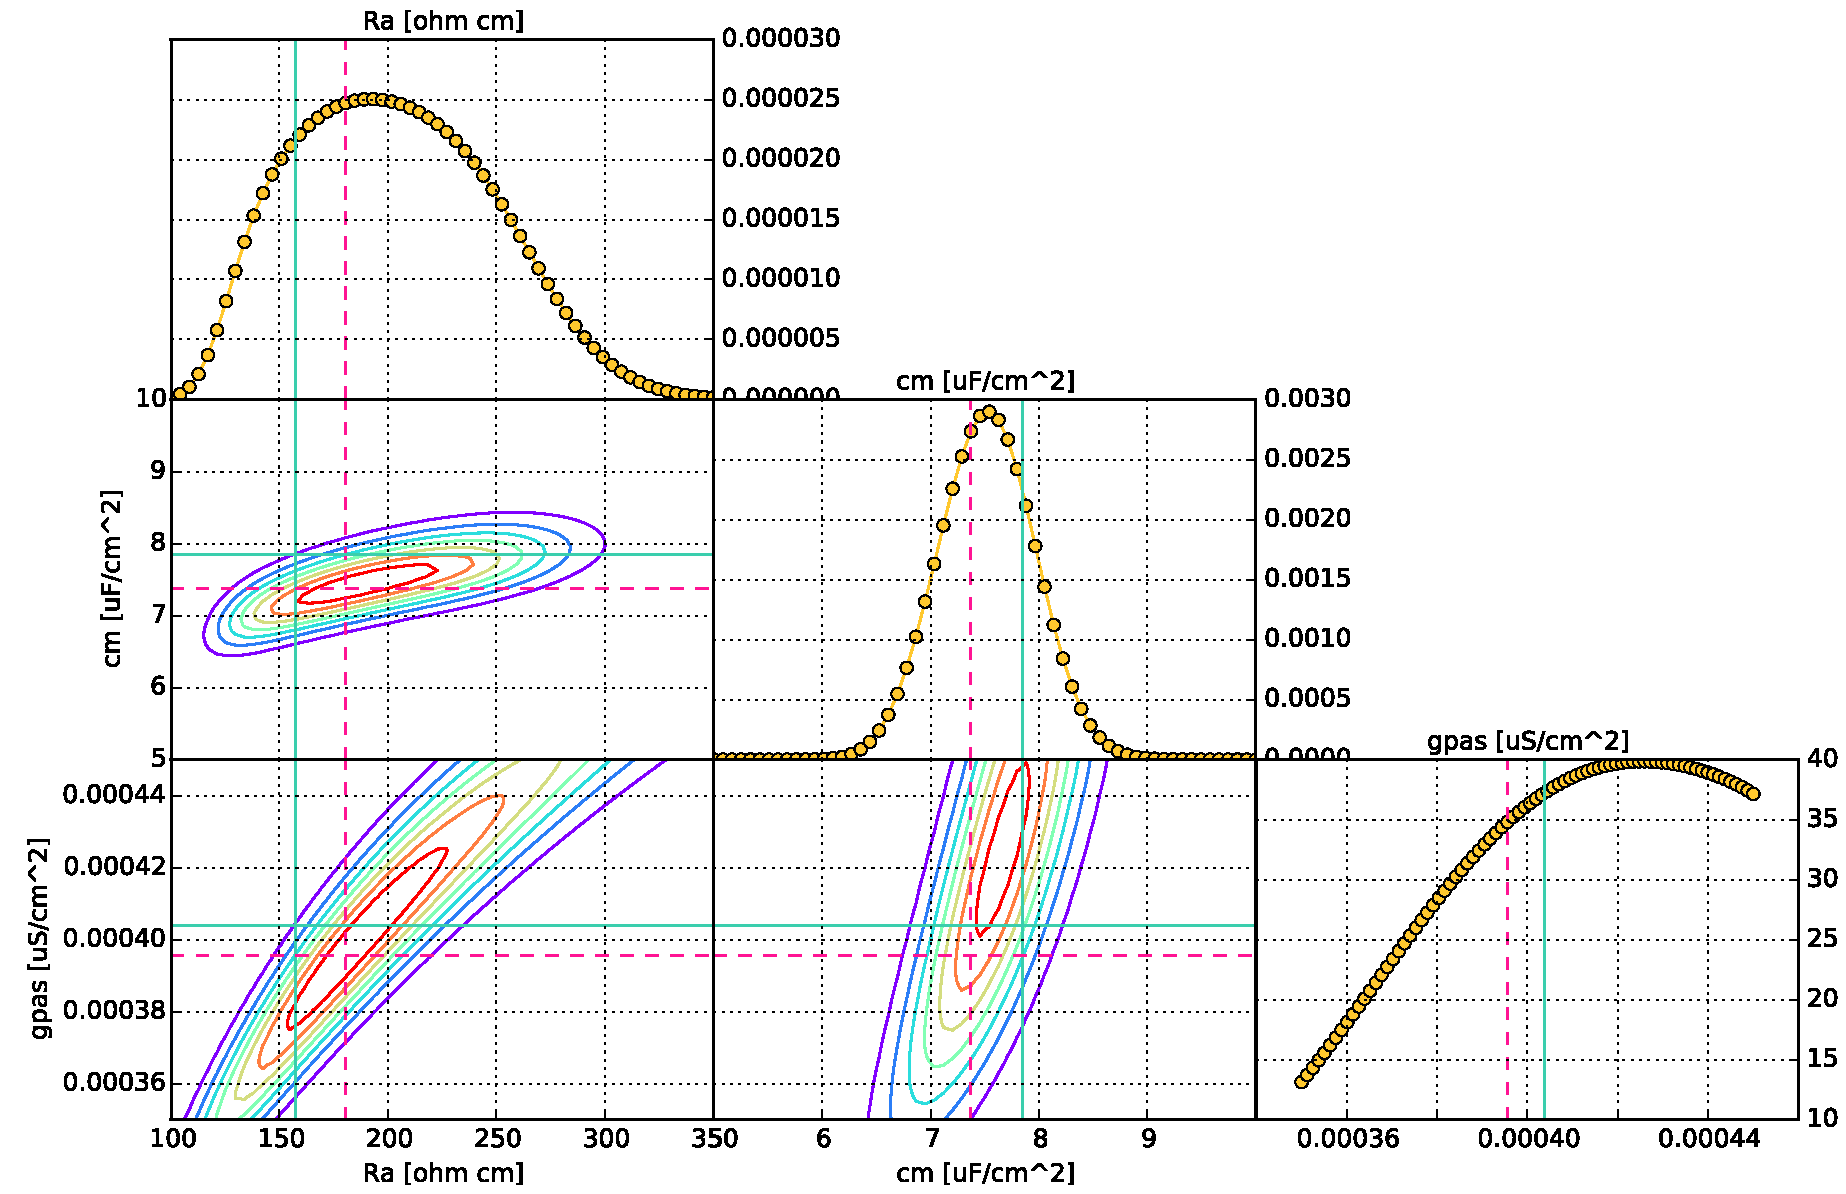
\includegraphics[width=\textwidth]{./fig/exp/fullplot_L(0).pdf} }}\\
	\subfloat[Poszterior eloszlás]{{\includegraphics[width=\textwidth]{./fig/exp/fullplot_P(0).pdf} }}
	\caption[Valós kísérleti adatsoron végzett inferencia összefoglaló ábrája]{Az összefoglaló ábra látható a paraméterbecslés eredményéről, valós passzív idegsejtre.}
	\label{fig:fullplot_res}
\end{figure}

